In this chapter, the implementation of four models for lithium-ion batteries is discussed, and their behavior in a co-simulation environment, depicting a data center's power system, is analyzed. Thereby, Section \ref{battery_models_for_co_simulation} introduces and parameterizes the used battery models, and Section \ref{experimental_results_and_discussion} discusses the experimental results of different scenarios.

\section{Battery Models for Co-Simulation}
\label{battery_models_for_co_simulation}


\subsection{SimpleBattery}
\subsection{CLCBattery}
\subsection{PybammBattery}
\subsection{LiionBatteryPack}
\begin{figure}[t]
    \centering
    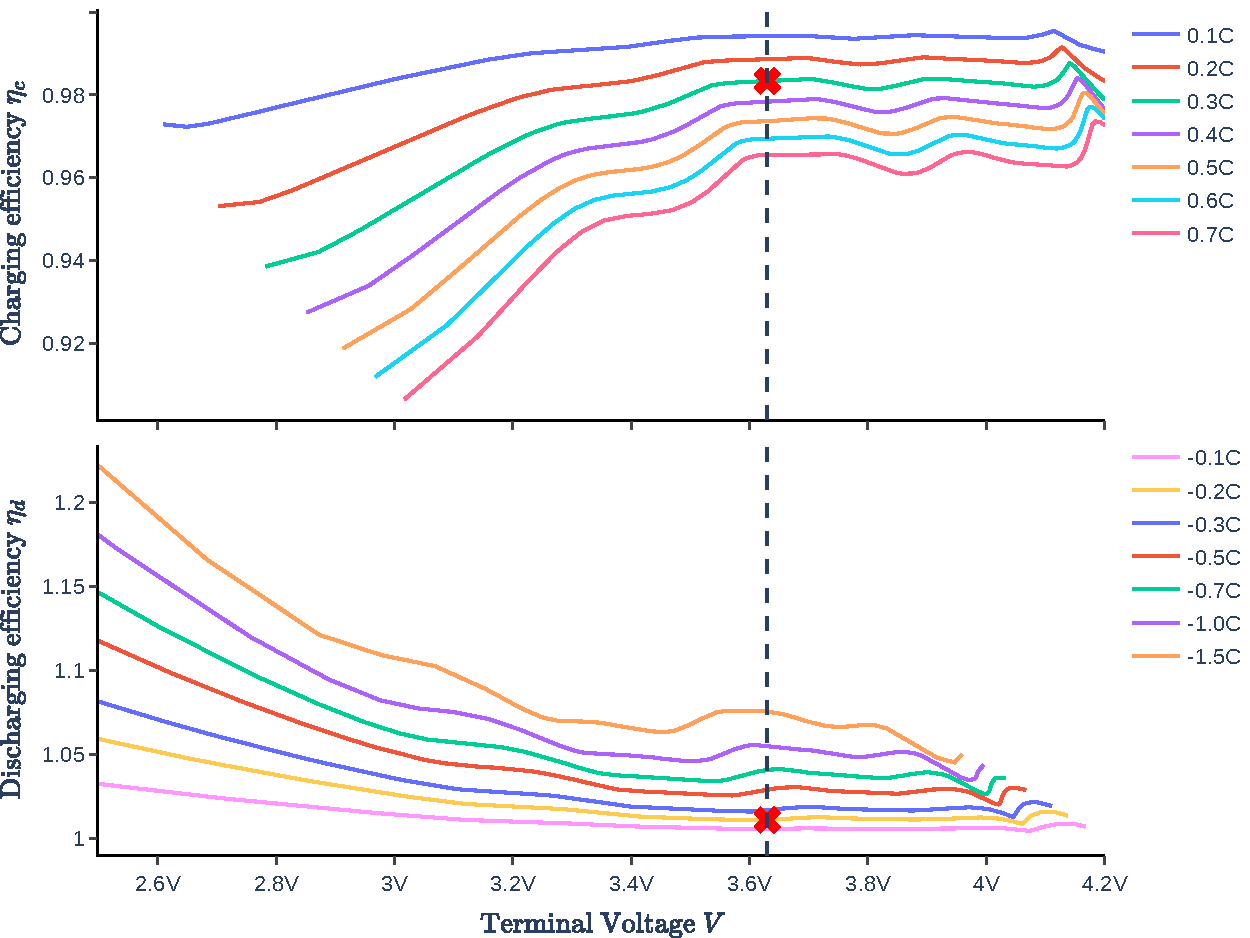
\includegraphics[width=\linewidth]{thesis/Images/charging_efficiency.pdf}
    \caption{Average charging efficiency}
    \label{fig:charging_efficiency}
\end{figure}
\begin{figure}[t]
    \centering
    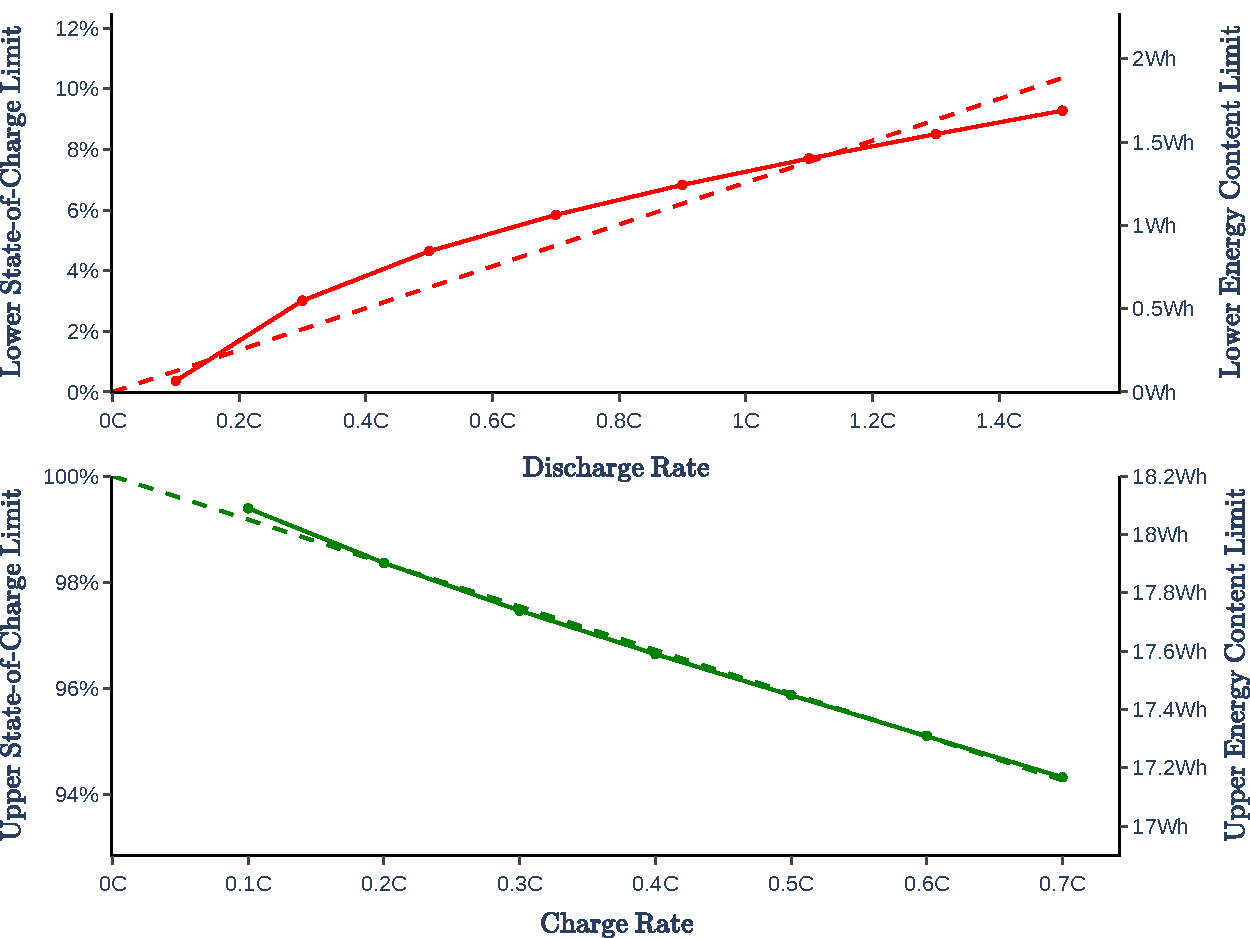
\includegraphics[width=\linewidth]{thesis/Images/energy_limits.pdf}
    \caption{Energy limits}
    \label{fig:energy_limits}
\end{figure}
\begin{figure}[t]
    \centering
    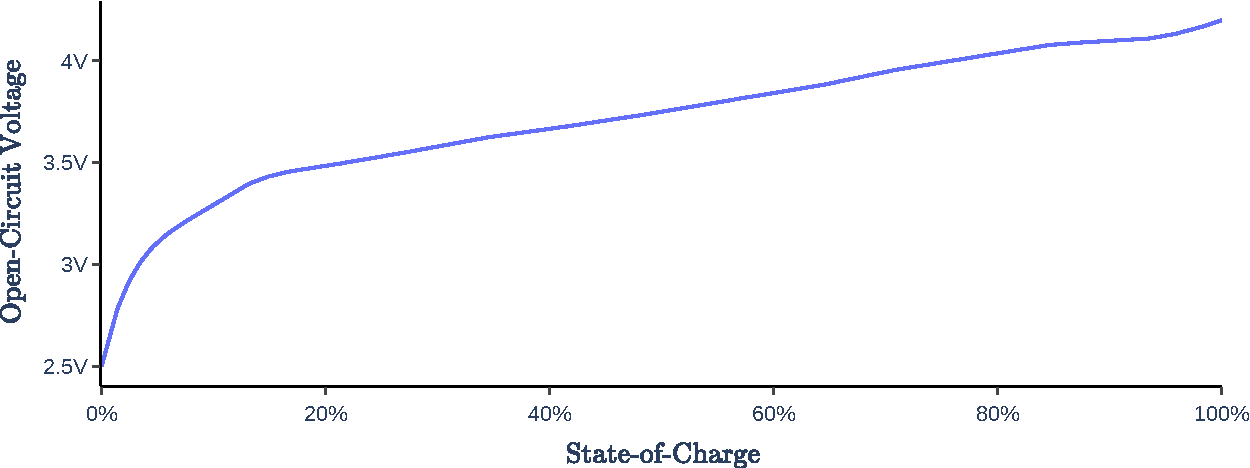
\includegraphics[width=\linewidth]{thesis/Images/soc_estimation.pdf}
    \caption{State-of-Charge estimation}
    \label{fig:soc_estimation}
\end{figure}
\begin{figure}[t]
    \centering
    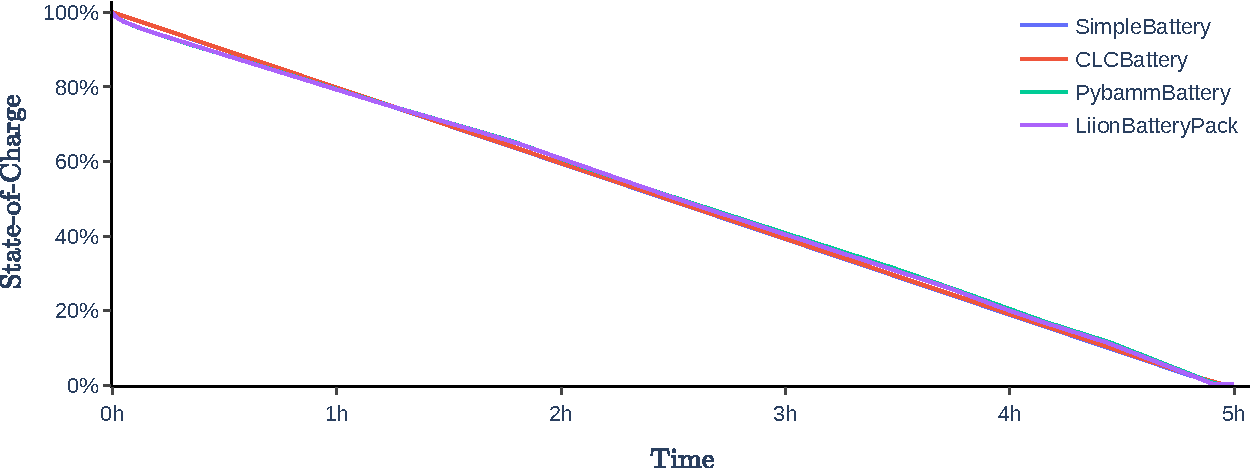
\includegraphics[width=\linewidth]{thesis/Images/discharge_energy.pdf}
    \caption{Discharge energy}
    \label{fig:discharge_energy}
\end{figure}
\section{Experimental Results and Discussion}
\label{experimental_results_and_discussion}
\begin{figure}[t]
    \centering
    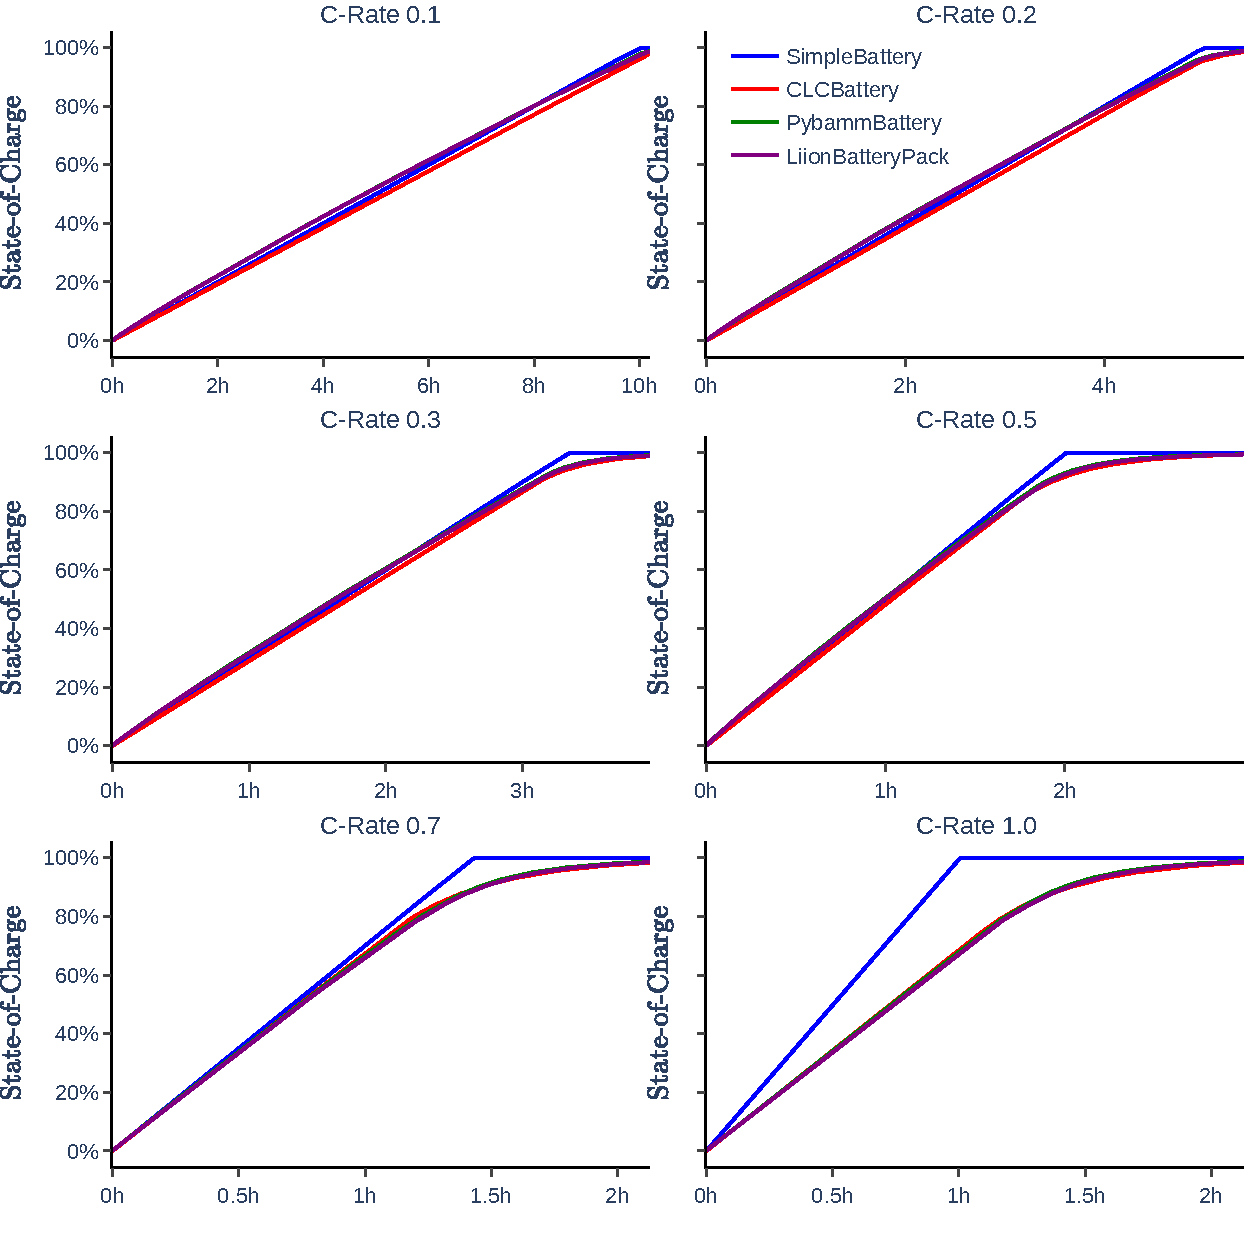
\includegraphics[width=\linewidth]{thesis/Images/charging_experiment.pdf}
    \caption{Charging Experiment}
    \label{fig:charging_experiment}
\end{figure}
\begin{figure}[t]
    \centering
    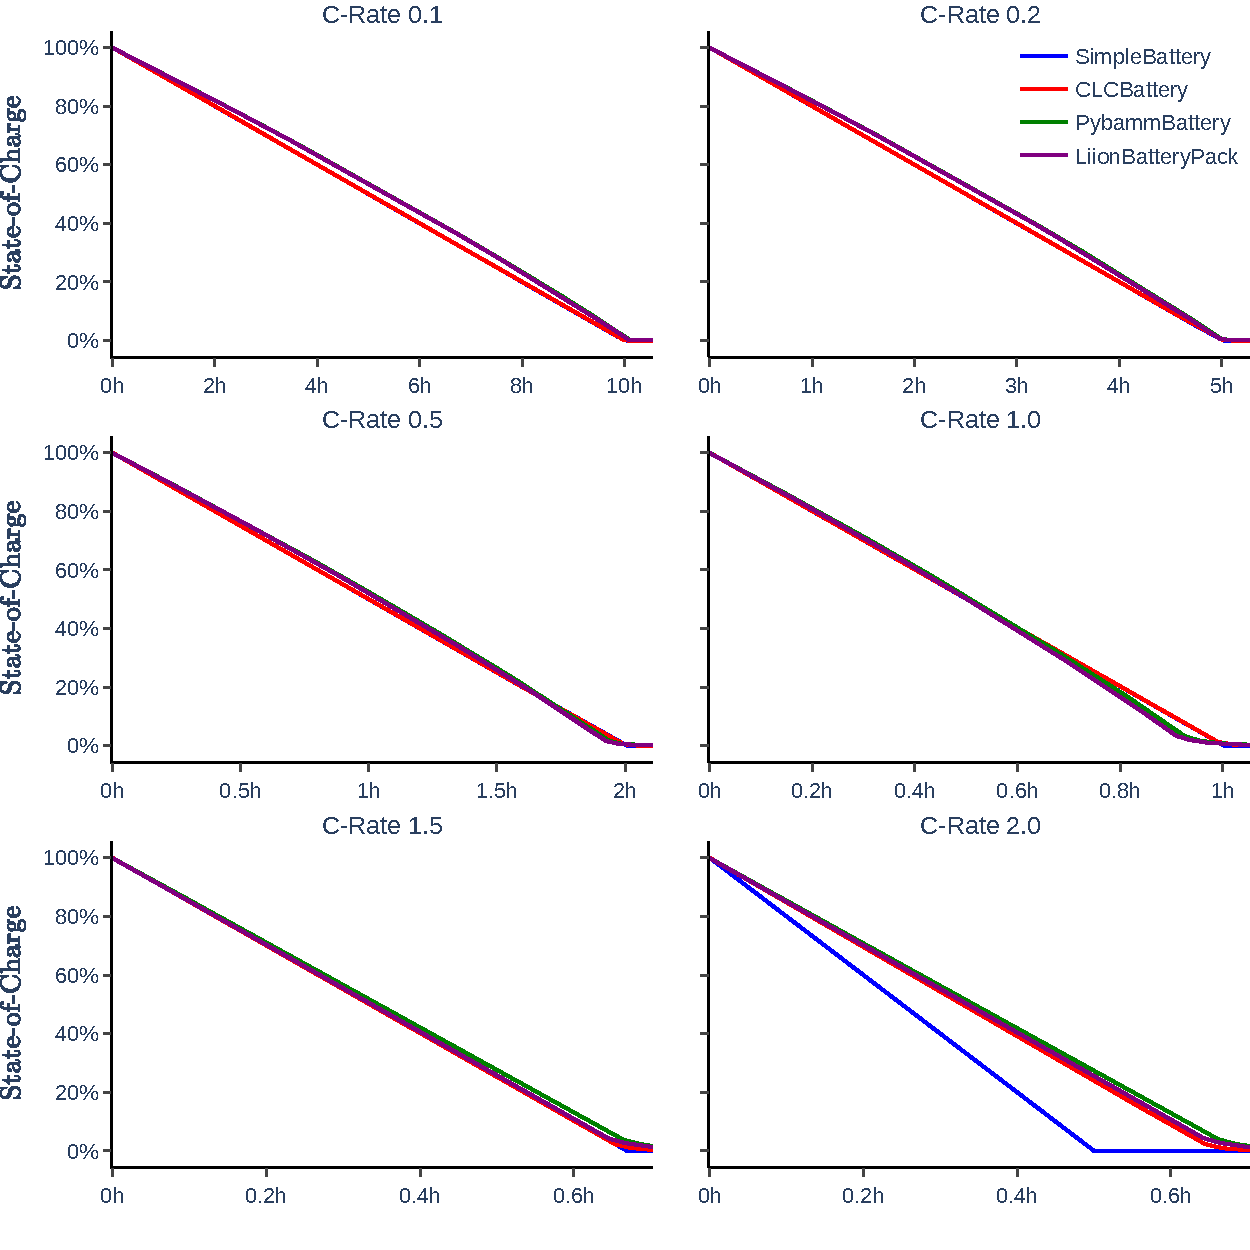
\includegraphics[width=\linewidth]{thesis/Images/discharging_experiment.pdf}
    \caption{Discharging Experiment}
    \label{fig:discharging_experiment}
\end{figure}